\documentclass[12pt]{article}
\usepackage{fullpage,amsmath,amssymb,graphicx}

\usepackage{setspace}
\spacing{1}

\usepackage{textpos}
\usepackage{tikz}
\usepackage{pgf}
\usepackage{amssymb}
\usepackage{enumerate}
\usepackage{xcolor}
\usepackage{graphicx}
\usepackage{subcaption}
\usepackage{tabularx}
\usepackage{colortbl}
\usepackage{multicol}
\usepackage{longtable}
\usepackage{hyperref}


\definecolor{encabezado}{rgb}{0.74, 0.83, 0.9}

\begin{document}

\hfill\\
\rule{\textwidth}{1.5pt}

\begin{minipage}[t]{85mm}
  \begin{tabular}{l}
    \textbf{\large Instituto Tecnológico de Costa Rica} \\  
    \textbf{Escuela de Ingeniería Electrónica} \\
    \textbf{Trabajo Final de Graduación} \\
    \textbf{Proyecto:} Método basado en aprendizaje reforzado \\para el control automático de una planta no lineal. \\
    \textbf{Estudiante:} Oscar Andrés Rojas Fonseca \hspace{3cm}\rule{4.5cm}{1.5pt}\\
    I Semestre 2024 \hspace{8.5cm}\textbf{Firma del asesor}
  \end{tabular}
\end{minipage}
\hfill\\
\rule{\textwidth}{1.5pt}


\section*{Bitácora de trabajo}

%\begin{table}[h]
\begin{minipage}[h]{\textwidth}
	\centering
	\begin{tabularx}{\textwidth}{|p{2cm}|X|X|p{2cm}|} 
		\hline
		\rowcolor{encabezado}
		\textbf{Fecha} & 
		\textbf{Actividad} & 
		\textbf{Anotaciones} & 
		\textbf{Horas dedicadas} \\ \hline
		% ***************************************************************
		05/02/2024 & 
		$\mathbf{1}.$ ADSASASAS. & 
		$a)$ CDCDCDCDCDC. \newline $b)$ VFVFVFVFV. \newline & 
		3 horas \\
	 	% ***************************************************************
	 	06/02/2024 & 
	 	$\mathbf{2}.$ ADSADASDASD. &
	 	$a)$ QWEQWEQ. \newline $b)$ CVBCVBCVBCVB. \newline & 
	 	3 horas \\
	 	% ***************************************************************
	 	06/02/2024 & 
	 	$\mathbf{3}.$ ASDASDASDA. & 
	 	$a)$ WQEQWEWQEQW. \newline $b)$ RDFDVFVDFV. \newline $c)$ HHJKHJKJK. & 
	 	3 horas \\
	 	
	 	\hline
	\end{tabularx}
\end{minipage}	 	
	 	
	 	% ***************************************************************
\hfill\\
\begin{minipage}[h]{\textwidth}
	\centering
	\begin{tabularx}{\textwidth}{|p{2cm}|X|X|p{2cm}|} 
		\hline		
		
	 	07/02/2024 & 
	 	$\mathbf{4}.$ ADADADAD & 
	 	$a)$ ADADADADAD. \newline $b)$ SFSFSFSFS. \newline & 
	 	5 horas \\
	 	% ***************************************************************
	 	09/02/2024 & 
	 	$\mathbf{5}.$ ADADADADADA. & 
	 	$a)$ SFSFSFSFSF.\newline $b)$ CSCSCSCS. \newline & 
	 	2 horas \\
	 	% ***************************************************************
	 	\hline
		\multicolumn{3}{|r|}{Total de horas de trabajo:} & 21 horas \\ 
	 	\hline                 
	\end{tabularx}
\end{minipage}
%\end{table}

% *****************************************************************************
% *****************************************************************************
% *****************************************************************************

\section*{Contenidos de actividades}

\subsection*{Resumen de teoría PAMH}

ADADADADADADADADADA
\cite{DataScience}

%\begin{figure}[h]
%	\centering
%	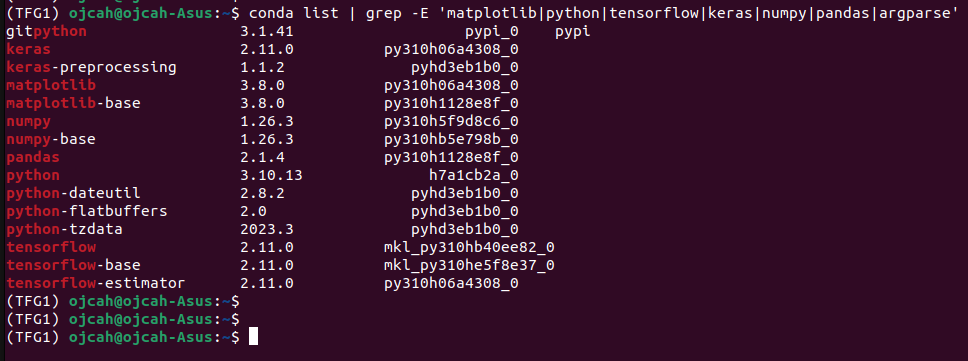
\includegraphics[scale=0.43]{Fig/CapturaEnv.png}
%	\caption{Lista simplificada de bibliotecas del \textit{environment} TFG1.}
%	\label{fig:capturaenv}
%\end{figure}



\newpage

\section*{Referencias}
\renewcommand\refname{}
\bibliographystyle{IEEEtran}
\bibliography{references}





\end{document}